\documentclass[runningheads]{llncs}

\usepackage{graphicx}
% Used for displaying a sample figure. If possible, figure files should
% be included in EPS format.
\usepackage{float}
\usepackage{appendix}

\begin{document}
	%
	\title{Scientific Paper}
	
	\author{Benjamin Vandersmissen\inst{1} \and
		Lars Van Roy\inst{2} \and \\
		Evelien Daems\inst{3} \and
		Frank Jan Fekkes\inst{4}}
	%
	\authorrunning{B. Vandersmissen, L. Van Roy, E. Daems, F.J. Fekkes}
	% First names are abbreviated in the running head.
	% If there are more than two authors, 'et al.' is used.
	%
	\institute{
		\email{benjamin.vandersmissen@student.uantwerpen.be} \and
		\email{lars.vanroy@student.uantwerpen.be} \and
		\email{evelien.daems@student.uantwerpen.be} \and
		\email{franciscus.fekkes@student.uantwerpen.be}}
	%
	\maketitle              % typeset the header of the contribution
	%
	\begin{abstract}
		This paper will give an in depth view of the performed adaptations to the Stride project, as well as an overview of the findings that were obtained by comparing these additions to the original stride project. 
		
		%\keywords{First keyword  \and Second keyword \and Another keyword.}
		
	\end{abstract}
	
	
	\section{Introduction}
	The stride project is designed to simulate and evaluate the lifetime of various infectious diseases. In order to properly analyze which factors have an effect on various diseases, the stride project allows multiple factors to be varied so that we can get an idea of which factors are the main influence  for the evolution of diseases. This expansion to the original stride project will include 2 major corrections, to make the simulation more realistic, being an improved workplace size distribution and an improved household composition distribution, a major addition to the pools in which diseases can spread, being daycare and preschool pools, a minor addition to make the input more variable by adding two addition input types being HDF5 and JSON and finally a visualizer that will allow users to get a graphical overview of where the diseases are most active, along with a list of parameters to give further information of the evolution of the disease for a given location. \\
	\\
	Other than these additions, there will also be a section about the simulation over entire Belgium, compared to isolated within Flanders. Other than just the simulated area, there will also be a comparison between the data derived from the Belgian population and the data derived from the Flemish population.
	
	\section{Daycare \& Preschool}
		In the original stride implementation, there are no specific contact pools for children aged 6 and under. The only way they could get infected was via the HouseHold contactpool. This is of course unrealistic. In this iteration of stride, 2 more contact pools are added, Daycare for children aged 0 to 3 and PreSchool for children aged 3 to 6. In this section, we discuss some of the repercussions of this change. \\ 
	\\
	Intuitively, by adding these contactpools, we should see that diseases spread faster than normal. To test this hypothesis, we generated a geopopulation with daycares and preschools and one without. Both are generated with the config file \textit{run\_generate\_default.xml} and then used them both in simulations.The result is shown in the following graph.
	\begin{figure}
			\centering
		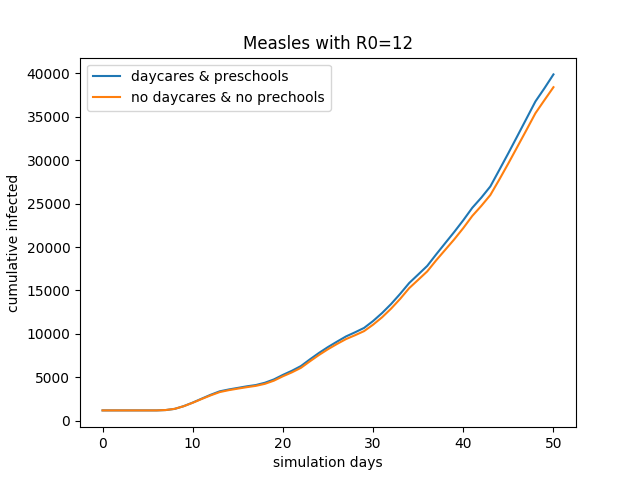
\includegraphics[width=0.9\textwidth]{measles_r12_daycare_comparison.png}	
		\caption{Average result of 10 simulations with and without daycares and preschools}
		\label{fig0}
	\end{figure}
	\\
	As shown in the graph, there are more infected persons with the implementation of daycares and preschools. With these parameters, there are around 2000 infected more after 50 days or a little more than 5\% extra infected.
	\section{Data Formats}
	\subsection{HDF5}
	HDF5 is a scientific dataformat specifically designed to store and organise large amounts of data. In this section, we compare the sizes of the fileformats already available in stride (protobuf and JSON) with the size of an HDF5 file and we also cover the write speed. Both these metrics are based on the configuration file \textit{run\_generate\_default.xml} with only the output file changed.
	\\
	As shown in table \ref{table:1}, HDF5 is memory-wise between protobuf and JSON. This is because protobuf is a heavily compressed format and HDF5 is not, but HDF5 isn't a plain text format like JSON either. In terms of write speed, HDF5 is a lot slower than Protobuf and JSON. A simple explanation for this is the fact that HDF5 does not support streams, while JSON and Protobuf do. This means that HDF5 has to write everything with it's own procedures which isn't as efficient. HDF5 does not support streams, because it was originally a C library, where streams did not exist and the C++ implementation is just a wrapper around the original C library.
	\begin{table}
		\centering
		\begin{tabular}{|c|c|c|}
			\hline
			\textbf{FileFormat} & \textbf{Size (Kb)}  & \textbf{Average write Time (s)}\\ \hline
			Protobuf & 13.713 & 1.74\\ \hline
			JSON & 317.050 & 5.25\\ \hline
			HDF5 & 125.066 & 30.45 \\ \hline
		\end{tabular}
		\caption{Performance of different data formats based on 10 runs of run\_generate\_default.xml}
		\label{table:1}
	\end{table}
	\section{Data Visualization}
	\section{Workplace Size Distribution}
	\subsection{Introduction}
	The original stride project made use of a set workplace size distribution, being an average size of 20, that would be randomly populated. So it might be that there would be smaller and larger workplaces, but the average would be around 20, which is not accurate. The majority of the workplaces are smaller than 20 and there are workplaces that are way larger than 20. It would therefore be more accurate to add an input file that would give a distribution of which workplace size occurs with which chance.

	\subsection{Impact}
	To proof whether or not this addition had a major impact, and to show the size of its impact, we ran a couple of simulations with different values for r0. The resulting graphs are displayed in the annex. Even though the difference isn't huge, we can generally conclude that it most definitely made the spreading go faster. At the end of the simulations, the number of infected people is generally about 4\% lower compared to using the newer workplace implementation. We can therefore conclude that the original workplace implementation was indeed incorrect, and gave slightly flawed results.
	\section{Household Composition Distribution}
	\subsection{Introduction}
	One more flaw of the original stride project, is that it had no regard for the differences in household size within smaller regions. It used one big input file, that would give the general household configuration over the entire simulation area (in this case Flanders) but there are significant differences between households over the different provinces. We therefore wanted to be able to specify household information for each province. \\
	\\
	Other than provinces, there are also significant differences between regular cities and major cities. We therefore added one extra household configuration for major cities, along with a file specifying which cities are considered to be major.
	\subsection{impact}
	To proof the impact of this addition, we did the same simulations we did for the workplace distribution addition. These plots, found in the annex, are different to the plots from workplaces in that they are not consistent in the effect that occurred. We can see significant effects in all three plots, but for r0 equal to 8 we see that the new implementation gives a far lower number of diseased people, where the other two show that the new implementation gives a slightly higher number of diseased people, compared to the original stride, spread over the two, the average is still a drop of 2\%. We can conclude that this change was significant and that there was indeed a flaw in the original stride implementation or, in other words, the differences between regions and cities are significant to the simulation.

	\newpage
	
	\section{Belgian Simulations}
	\subsection{Introduction}
	To perform a simulation based on the current profile of the Belgian data, we searched for suitable numbers and studies that would give us reliable data to perform a simulation on the Belgian area.
	We didn't limit ourselves in this study to the Belgian population as a whole but we compared it to the fraction of the Flemish district as an area on its own.
	By doing two different studies, we can evaluate if the Flemish situation differs in a simulation when isolated or as a part of Belgium.
	
	This is an interesting point to study because one can ask himself the question if traffic in and out Flanders has a large influence or is it impact minimal and the most traffic is within the Flandrian area itself? Is the region very susceptible to the measles or are the measurements to prevent outbreaks well organized?
	
	Recently there has been a lot of reports that there has been an outbreak of measles in Europe and there have been reports of an outbreak in Belgium. It is a disease that can cause symptoms to young individuals but just as well to older ones who didn't get the vaccination when it was not mandatory. We think that is interesting to make simulations based on this disease because it is something current and is a reason for a lot of worrying within the health department.
	
	\subsection{Data about the region and disease}
	
	\subsubsection{Flanders} 
	The region of Flanders consists of a population of 6.550.000 people ~\cite{1}, which is a little bit more than half of the entire Belgian population. Most of the population we consider with a very high immunity rate. We could not find any scientific data to back out choice for a rate equal to 90\%. But we thought this was a good estimate since the vaccine rate in Flanders is quite high with its 96,2\%. This statistic in combination with the fact that vaccination against measles is obligatory in Belgium made us pretty confident to use a high immunity factor. ~\cite{2} ~\cite{3} ~\cite{4}\\
	
	We generated random households based on the average distribution of the household throughout Flanders.~\cite{5} The other files in the configuration were already provided with the original version of Stride and we did not alter this information. When looking at the number of people that are categorized as a student or as someone part of a workplace we found different sources that lead to a good estimate of these parameters. For the percentage of students, we found that approximately 49,5\% of the population is located in higher education.~\cite{6}~\cite{17} The number of people working is higher than the number of students with a value of 75.91\%.~\cite{7}
	\newpage
	\subsubsection{Belgium}
	
	Belgium has a population of 11.376.070 individuals ~\cite{8} and is quite a large number to run a lot of simulations. Therefore we performed 10 simulation runs using the Stan option. A large population is less susceptible for stochastic deviations and thus it can do no harm that we don't use 50 simulations or more to get an overall view of what will happen.\\
	
	As mentioned before, we studied an outbreak of the measles during a year in this context. And since the vaccination against measles is one of the mandatory vaccinations in Belgium, a rather high vaccine rate is used with a value of 90\%. ~\cite{9} In Belgium there is quite a large percentage of people who commute to work and have to travel outside their hometown. The population that we consider to be active and has a job takes up about 71.89\% of the entire population.~\cite{14} And we computed based on different statistics that the workplace commuting percentage had a value of approximately 0.644.~\cite{12} As for the students, they form a smaller percentage of the population than the working community with 45\%. (This is an approximated value because the graph did not contain any specific numbers.~\cite{15})\\
	
	To create a Belgian population based on data found in official governments databanks, we use some files containing the essential information. For the (provided) commuting data we had to alter the reader for the commuting information. We made this choice because it was much less effort to alter the code than to interpret the entire dataset and convert it to the same structure as other files. In the commuting information from Belgium, the proportions were already calculated and thus less work was needed to create this information since we only had to extract it. The data describing the households within Belgium is based on numbers we collected from studies which gave an insight into the size of the households in Belgium. Based on these numbers and on the proportion of different age categories, we created a random set of households for Belgium.~\cite{10} ~\cite{11}
	
	\subsection{Flanders vs. Belgium}
	
	In this section, we want to discuss the simulation results between a measles outbreak during one year in the country of Belgium and the Flanders region as an isolated area. The data we collected for this simulation was discribed in the previous section and now we want to discuss and evaluate some discoveries, remarks and findings. The graphs for this discussion can be found in Figure 13 and Figure 16 in the appendix.\\
	
	The first thing that we can immediately notice is that the simulation of Belgium creates a higher amount of infected people. Because the population within the region of Flanders is smaller than the population within Belgium we did expect a less small amount of infected people. In Flanders we have an average of 200 infected cases for 10 stochastic simulation runs over a time period of one year. This is a realistic value for an outbreak of the measles. We have found articles that state that there were 25 cases in the month of January of this year.~\cite{18}~\cite{13} In the graphical representation of the number of the infected count, we can see a large outbreak in the beginning and a flat line after 50 days. This can be explained by the high standards of vaccination in this region. Almost the entire Flandrian population has received a vaccination against the measles and once this vaccine has been taken you are as good as immune against the disease. The high spread, in the beginning, can not be avoided because it is a highly infectious disease and there is a group of people that didn't take the precautions like children younger than one year or individuals who can not receive the vaccine due to medical reasons.~\cite{20} 
	For Belgium, we can observe a different kind of increase. The number of infected count in Belgium is 2831. In Belgium, the spreading of the measles and the growing of the number of infected people increases more in value throughout the whole period of time rather than in a short window of time within the year as is the case in Flanders. But the growth rate is not as high as it is Flanders. The curve is more rounded upwards instead of being almost straight up as in Flanders. A reason for this is the larger population in Belgium. There is a larger percentage of unvaccinated people who move through a larger area. So it takes longer for everyone who can be infected to be effectively carrier of the disease. Having only 2831 cases of measles over a population of around 11 million people may seem a bit strange. But again this is due to the mandatory vaccination and a high vaccination rate.\\
	
    And lastly, we consider Flanders as a part of Belgium and it gives a higher average infected count of 260 for the Flandrian area. It is not such a big difference with the average of Flanders. There is now higher traffic of commuters in the region of Flanders because there can be individuals who live in Wallonia but work in the Flandrian region. The vaccination rate in Wallonia is slightly lower than in Flanders, this can also have an impact on the spreading of the disease.
	
	
	\newpage
	\begin{thebibliography}{20}
		\bibitem{1}
		Population of Flanders \\
		\url{https://www.statistiekvlaanderen.be/bevolking-omvang-en-groei}
		\\
		
		\bibitem{2}
		Vaccination rate in Europe \\
		\url{http://www.europarl.europa.eu/news/nl/headlines/society/20180316STO99921/vaccinatie-zorg-om-de-te-lage-vaccinatiegraad-in-de-eu}
		\\
		
		\bibitem{3}
		Measles: vaccination information \\
		\url{https://epidemio.wiv-isp.be/ID/Pages/Rougeole.aspx}
		\\
		
		\bibitem{4}
		Vaccination Flanders \\
		\url{https://www.zorg-en-gezondheid.be/nieuwe-cijfers-tonen-hoge-vaccinatiegraad-bij-vlamingen}
		\\
		
		\bibitem{5}
		Household size statisic chart (Flanders) \\
		\url{https://www.wonenvlaanderen.be/sites/wvl/files/wysiwyg/huishoudens\_naar\_hh-grootte.pdf}
		\\
		
		\bibitem{6}
		Education Flanders \\
		\url{https://www.vlaanderen.be/publicaties/vlaams-onderwijs-in-cijfers-2017-2018}
		
		\bibitem{7}
		Working population within Belgium \\
		\url{http://projecties.steunpuntwerk.be/werkzaamheid/tls/werkzaamheid/index.php}
		\\
		
		\bibitem{8}
		Structure of population Belgium \\
		\url{https://statbel.fgov.be/nl/themas/bevolking/structuur-van-de-bevolking\#news}
		\\
		
		\bibitem{9}
		Epidemics: Measles in Europe and Belgium 2017 \\
		\url{https://www.vaxinfopro.be/spip.php?article2249\&lang=nl\&retour=1}
		\\
		
		\bibitem{10}
		Household composition in Belgium \\
		\url{https://statbel.fgov.be/sites/default/files/Over\_Statbel\_FR/Sociaal-Economische\%20Enqu\%C3\%AAte\%202001\%20-\%20monografie\%204-Huishoudens\%20en\%20gezinnen\%20in\%20Belgi\%C3\%AB.pdf}	
		\\
		
		\bibitem{11}
		Age pyramid of Belgium \\
		\url{https://statbel.fgov.be/nl/themas/bevolking/structuur-van-de-bevolking\#panel-11}
		\\
		
		\bibitem{12}
		Commuting workplaces 2011 \\
		\url{http://www.census2011.be/analyse/flux\_nl.html}
		\\
		
		\bibitem{13}
		Number of reported measle cases in Flanders/Belgium \\
		\url{https://www.vaxinfopro.be/spip.php?article2938\&lang=nl}
		\\
		
		\bibitem{14}
		Employment and unemployment Belgium \\
		\url{https://statbel.fgov.be/nl/themas/werk-opleiding/arbeidsmarkt/werkgelegenheid-en-werkloosheid}
		\\
		
		\bibitem{15}
		Education policy profile (page 16) \\
		\url{http://www.oecd.org/education/Education-Policy-Outlook-Country-Profile-Belgium.pdf}
		\\
		
		\bibitem{16}
		Population stated by age in Flanders \\
		\url{https://www.statistiekvlaanderen.be/bevolking-naar-leeftijd-en-geslacht}
		\\
		
		\bibitem{17}
		Profile of number of students \\
		\url{https://www.werk.be/sites/default/files/rapporten/wse\_2-09\_jongeren\_in\_beeld-jan2009.pdf}
		\\
		
		\bibitem{18}
		Article about measles outbreak (De Standaard) \\
		\url{https://www.standaard.be/extra/pdf/belgieblootgelegd/BB7/BB7pagina6.pdf}
		\\
		
		\bibitem{19}
		Vaccination rate Flanders 2016 \\
		\url{https://www.zorg-en-gezondheid.be/sites/default/files/atoms/files/VIB\%202017-2\%20-\%20Vaccinatiegraad\%20in\%20Vlaanderen\%20in\%202016.pdf}
		\\
		
		\bibitem{20}
		All round info about the vaccination against measles \\
		\url{https://www.cm.be/ziekte-en-behandeling/vaccinaties/basisvaccinaties/mazelen}
		
	\end{thebibliography}
	
	
	\appendix
	\appendixpage
	\section{Workplace Size Distribution}
	\begin{figure}
		\centering
		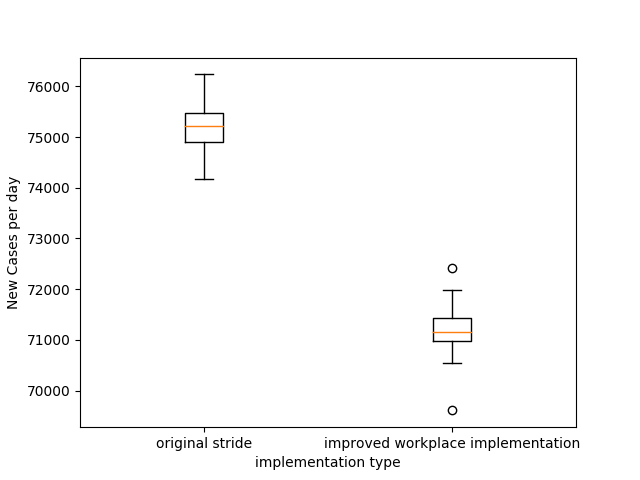
\includegraphics[width=0.9\textwidth]{workplace_r08_boxplot.png}	
		\caption{The boxplot for the different workplace implementations, using r0 equal to 8}
		\label{fig1}
	\end{figure}
	\begin{figure}
		\centering
		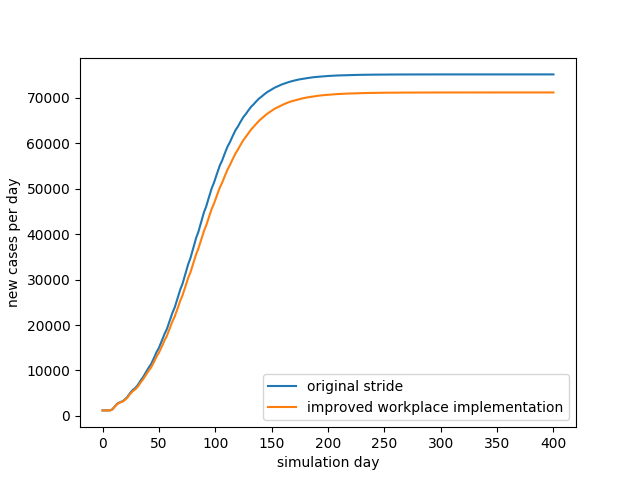
\includegraphics[width=0.9\textwidth]{workplace_r08_cumul.png}
		\caption{The cumulative evolution of the diseased people, using the different workplace implementations and r0 equal to 8}	
		\label{fig2}
		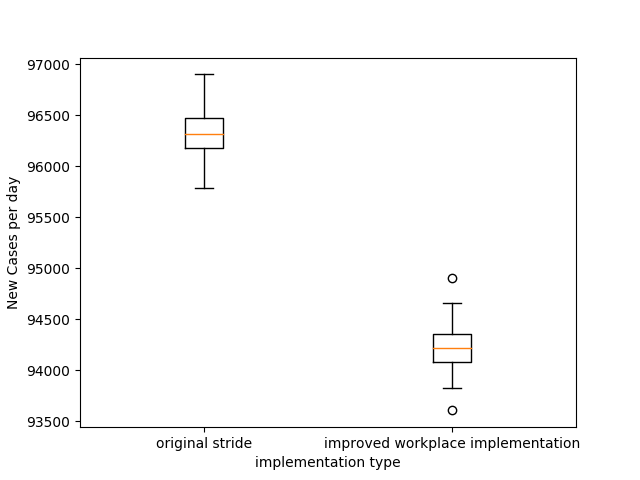
\includegraphics[width=0.9\textwidth]{workplace_r11_boxplot.png}	
		\caption{The boxplot for the different workplace implementations, using r0 equal to 11}
		\label{fig3}
	\end{figure}
	\begin{figure}
		\centering
		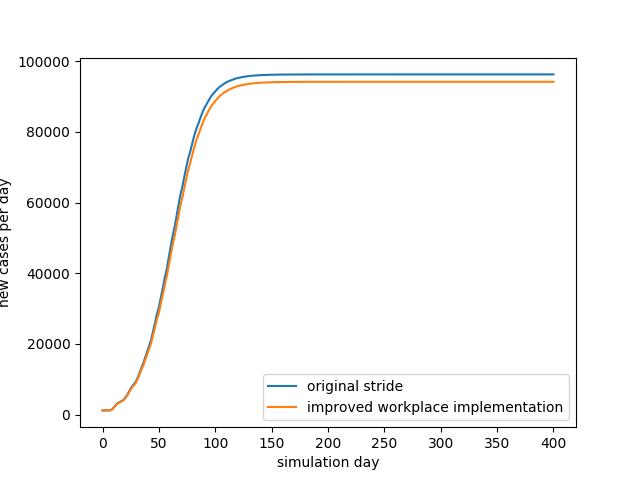
\includegraphics[width=0.9\textwidth]{workplace_r11_cumul.png}
		\caption{The cumulative evolution of the diseased people, using the different workplace implementations and r0 equal to 11}	
		\label{fig4}
		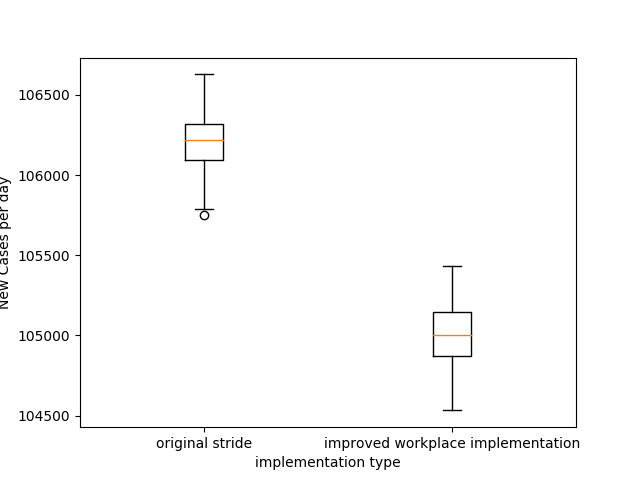
\includegraphics[width=0.9\textwidth]{workplace_r14_boxplot.png}	
		\caption{The boxplot for the different workplace implementations, using r0 equal to 14}
		\label{fig5}
	\end{figure}
	\begin{figure}
		\centering
		\centering
		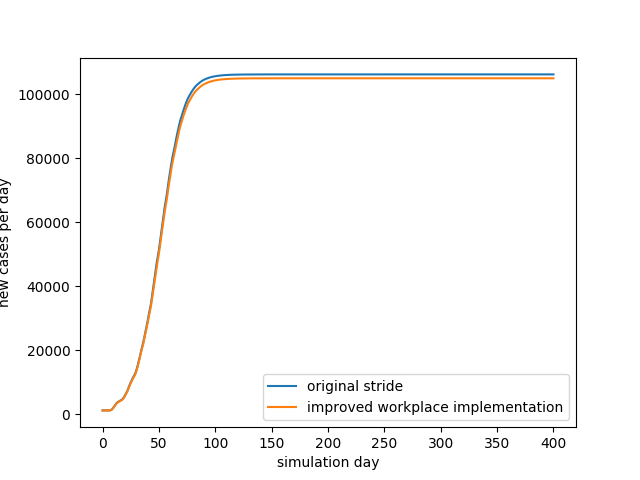
\includegraphics[width=0.9\textwidth]{workplace_r14_cumul.png}
		\caption{The cumulative evolution of the diseased people, using the different workplace implementations and r0 equal to 14}	
		\label{fig6}
	\end{figure}
	\clearpage
	\section{Household Composition Distribution}
	\begin{figure}
		\centering
		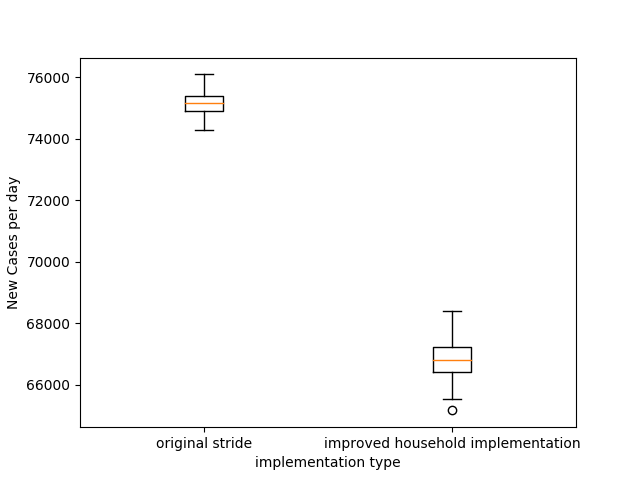
\includegraphics[width=0.9\textwidth]{household_r08_boxplot.png}	
		\caption{The boxplot for the different household implementations, using r0 equal to 8}
		\label{fig7}
	\end{figure}
	\begin{figure}
		\centering
		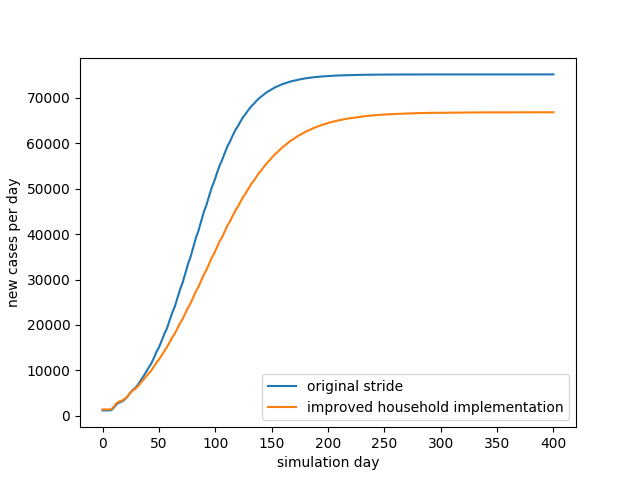
\includegraphics[width=0.9\textwidth]{household_r08_cumul.png}
		\caption{The cumulative evolution of the diseased people, using the different household implementations and r0 equal to 8}	
		\label{fig8}
		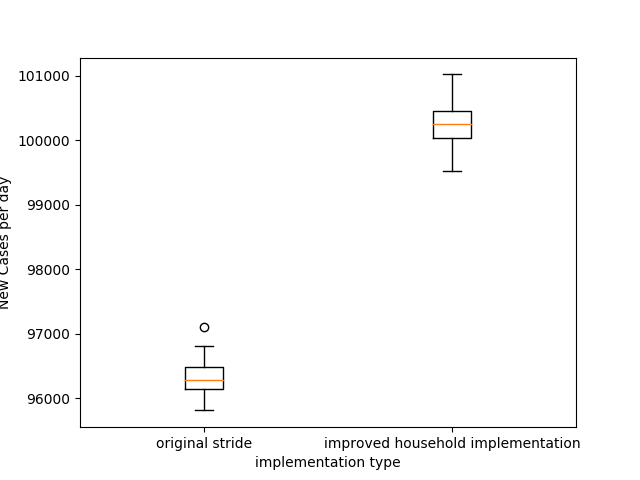
\includegraphics[width=0.9\textwidth]{household_r11_boxplot.png}	
		\caption{The boxplot for the different household implementations, using r0 equal to 11}
		\label{fig9}
	\end{figure}
	\begin{figure}
		\centering
		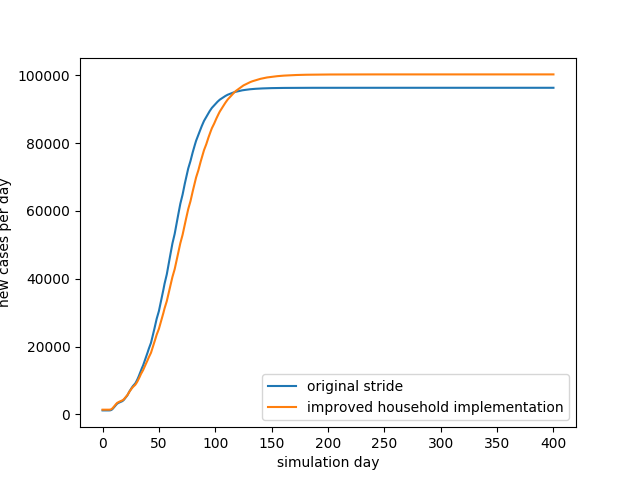
\includegraphics[width=0.9\textwidth]{household_r11_cumul.png}
		\caption{The cumulative evolution of the diseased people, using the different household implementations and r0 equal to 11}	
		\label{fig10}
		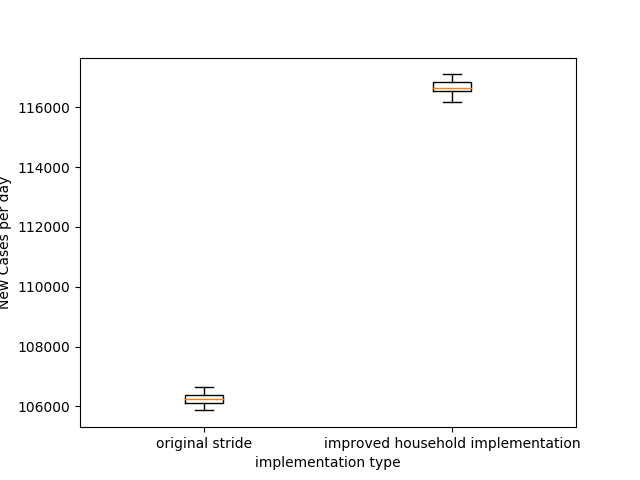
\includegraphics[width=0.9\textwidth]{household_r14_boxplot.png}	
		\caption{The boxplot for the different household implementations, using r0 equal to 14}
		\label{fig11}
	\end{figure}
	\begin{figure}
		\centering
		\centering
		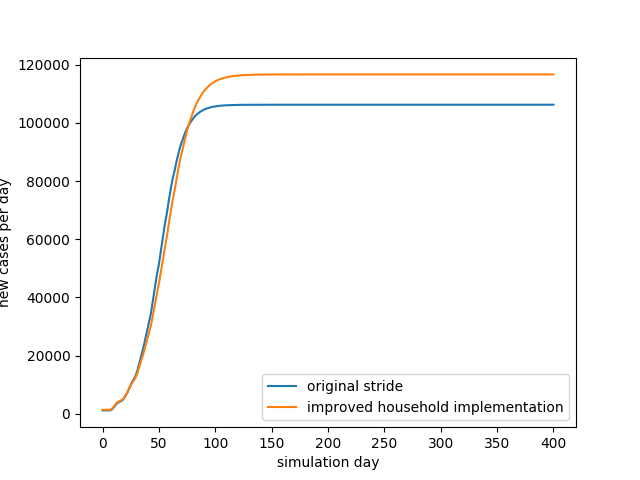
\includegraphics[width=0.9\textwidth]{household_r14_cumul.png}
		\caption{The cumulative evolution of the diseased people, using the different household implementations and r0 equal to 14}	
		\label{fig12}
	\end{figure}
	\begin{figure}
		\centering
		\centering
		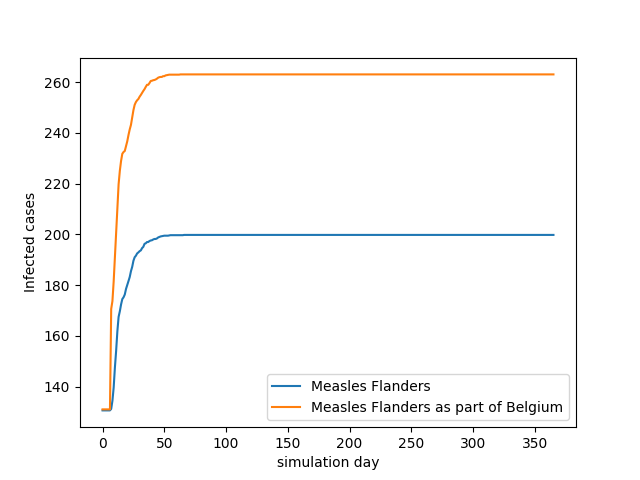
\includegraphics[width=0.9\textwidth]{FL1_FL2_sim_infected.png}
		\caption{The cumulative evolution of the diseased people (Flanders as an isolated area and as part of Belgium)}	
		\label{fig13}
	\end{figure}
	\begin{figure}
		\centering
		\centering
		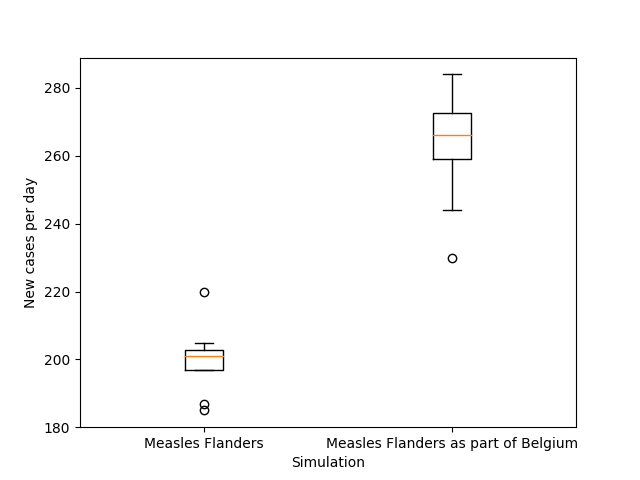
\includegraphics[width=0.9\textwidth]{FL1_FL2_sim_boxplot.png}
		\caption{The boxplot of the diseased people (Flanders as an isolated area and as part of Belgium)}	
		\label{fig14}
	\end{figure}
	\begin{figure}
		\centering
		\centering
		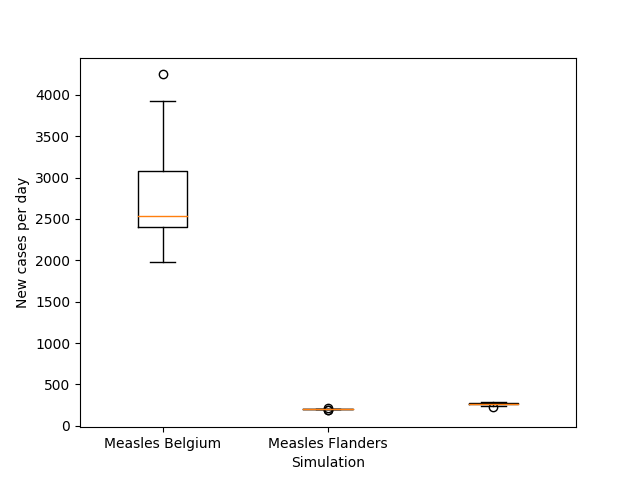
\includegraphics[width=0.9\textwidth]{BE_sim_boxplot.png}
		\caption{The boxplot of the diseased people (Flanders and Belgium)}	
		\label{fig15}
	\end{figure}	
	\begin{figure}
		\centering
		\centering
		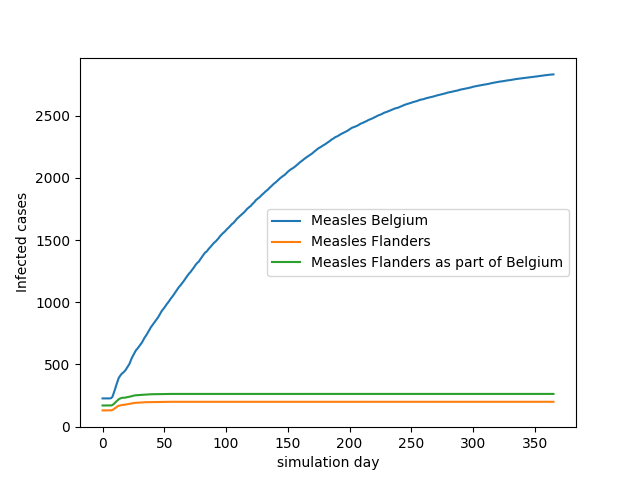
\includegraphics[width=0.9\textwidth]{BE_sim_infected_cases.png}
		\caption{The boxplot of the diseased people (Flanders and Belgium)}	
		\label{fig16}
	\end{figure}

\end{document}

